\subsection{Евклидовы кольца и деление с остатком}

\begin{definition}
	Область целостности $K$ называется \textit{евклидовым кольцом}, если определена функция $N: K\backslash\{0\} \to \N \cup \{0\}$, называемая \textit{нормой}, удовлетворяющая условиям:
	\begin{enumerate}
		\item $\forall a, b \in K\backslash\{0\}: N(ab) \ge N(a)$
		\item $\forall a, b \in K\backslash\{0\}: \exists q, r \in K: a = bq + r$, где $r = 0$ или $N(r) < N(b)$ ($q$ называется \textit{частным}, а $r$ "--- \textit{остатком} при делении $a$ на $b$)
	\end{enumerate}
\end{definition}

\begin{note}
	Первое свойство в определении выше не является обязательным. Кроме того, часто его заменяют на неэквивалентное свойство $\forall a, b \in K \backslash \{0\}: N(ab) = N(a)N(b)$.
\end{note}

\begin{note}
	Любое поле является евклидовым кольцом: норму в поле можно положить тождественно равной 0 или 1, поскольку при делении в поле остаток всегда равен $0$.
\end{note}

\begin{example}
	Рассмотрим несколько примеров евклидовых колец:
	\begin{enumerate}
		\item $\Z$ "--- евклидово кольцо с нормой $\forall z \in \Z: N(z) = |z|$.
		\item Если $F$ "--- поле, то $F[x]$ "--- евклидово кольцо с нормой $\forall p \in F[x]: N(p) = \deg{p}$ (причем если положить норму равной $2^{\deg{p}}$, выполняться будет даже более сильное мультипликативное условие).
		\item $\Z[i]$ "--- евклидово кольцо с нормой $\forall z \in \Z[i]: N(z) = |z|$. Докажем это геометрически. Пусть $a, b \in \Z[i] \backslash \{0\}$. Число $\frac ab$ попадает в квадрат со стороной 1 на комплексной плоскости, поэтому достаточно выбрать в качестве $q$ вершину этого квадрата, ближайшую к $\frac ab$, тогда $r = a - bq$, и $N(r) = N(\frac ab - q)N(b) \le \frac12N(b)$. Это рассуждение проиллюстрировано ниже:
		\begin{center}
			\scalebox{1}{
				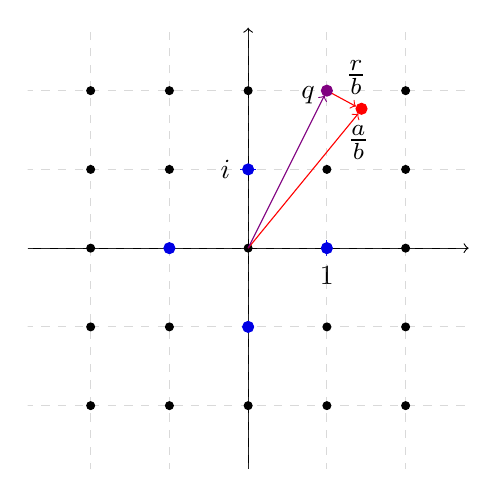
\begin{tikzpicture}
					\clip (-2.8, -2.8) rectangle (2.8, 2.8);
					\draw [->] (-2.8, 0) -- (2.8, 0);
					\draw [->] (0, -2.8) -- (0, 2.8);
					
					\draw [blue] (1,3pt) -- (1,-3pt) node [below, black] {$1$};
					\draw [blue] (3pt,1) -- (-3pt,1) node [left, black] {$i$};
					\draw[style=help lines,dashed, thin, gray, opacity=0.3] (-6,-6) grid (6,6);
					
					\foreach \x in {-5, -4, ..., 5}{
						\foreach \y in {-5, -4, ..., 5}{
							\node[draw,circle,inner sep=1pt,fill] at (\x, \y) {};
						}
					}
					
					\draw [->, red] (0, 0) -- (1.4, 1.71) node [black, below, scale = 1.2] {$\frac ab$};
					\draw [->, red] (1, 2) -- (1.37, 1.8) node [black, above, scale = 1.2] {$\frac rb$};
					\draw [->, violet] (0, 0) -- (0.97, 1.94) node [black, left] {$q$};
					\node[draw,circle,inner sep=1.4pt,fill,black!10!blue] at (0, 1) {};
					\node[draw,circle,inner sep=1.4pt,fill,black!10!blue] at (1, 0) {};
					\node[draw,circle,inner sep=1.4pt,fill,black!10!blue] at (0, -1) {};
					\node[draw,circle,inner sep=1.4pt,fill,black!10!blue] at (-1, 0) {};
					
					\node[draw,circle,inner sep=1.4pt,fill,red] at (1.44, 1.77) {};
					\node[draw,circle,inner sep=1.4pt,fill,violet] at (1, 2) {};
				\end{tikzpicture}
			}
		\end{center}
	
		Доказать евклидовость $\Z[i]$ можно и алгебраически. Пусть $\frac ab = \alpha + \beta i, \alpha, \beta \in \Q$. Выберем $A, B \in \Z$ "--- целые числа, ближайшие к $\alpha, \beta$ соответственно. Тогда, если положить $q := A + Bi$, то $r = a - qb$, и $N(\frac{r}{b}) = (\alpha - A)^2 + (\beta - B)^2 \le \frac1{2^2} + \frac1{2^2} < 1$, откуда $N(r) < N(b)$.
	\end{enumerate}
\end{example}

\begin{note}
	Оба доказательства евклидовости $\Z[i]$, приведенные выше, могут быть применены к кольцам $\Z[\omega]$, $\Z[\sqrt{2}i]$.
\end{note}

\begin{proposition}
	В определении евклидова кольца достаточно требовать от нормы только свойство деления с остатком: $\forall a, b \in K\backslash\{0\}: \exists q, r \in K: a = bq + r$, где $r = 0$ или $N(r) < N(b)$.
\end{proposition}

\begin{proof}
	Пусть $K$ "--- область целостности, $N: K \backslash \{0\} \to \N \cup \{0\}$ "--- функция со свойством деления с остатком. Для $\forall a \in K \backslash \{0\}$ положим $\overline{N}(a) := \min\{N(ab) : b \in K \backslash \{0\}\}$. Проверим, что для $\overline{N}$ выполнены оба свойства нормы:
	\begin{enumerate}
		\item Заметим, что $\forall a, b \in K \backslash \{0\}: \overline{N}(ab) = N(abc)$ для некоторого $c \in K \backslash \{0\}$. Тогда $\overline{N}(ab) \ge \min\{N(ax) : x \in K \backslash \{0\}\} = \overline{N}(a)$.
		\item Пусть $a, b \in K \backslash \{0\}$. Выберем такой $x \in K \backslash \{0\}$, что $\overline{N}(b) = N(bx)$, и поделим $a$ на $bx$ с остатком: $a = bxq + r$, где либо $r = 0$, либо $N(r) < N(bx)$. Остается заметить, что тогда $\overline{N}(r) \le N(r) < N(bx) = \overline{N}(b)$.\qedhere
	\end{enumerate}
\end{proof}

Теперь \textbf{до конца раздела} зафиксируем евклидово кольцо $K$.

\begin{proposition}
	У каждого элемента $x \in K \backslash \{0\}$ существует разложение.
\end{proposition}

\begin{proof}
	Предположим, что это не так и рассмотрим элемент $x \in K \backslash \{0\}$ с минимальной нормой, который не раскладывается в произведение неразложимых. Представим $x$ в виде $x = ab$, где $a, b \in K \backslash \{0\}$, тогда $N(x) \ge N(a)$, $N(x) \ge N(b)$.
	
	Если оба неравенства строгие, то разложение элемента $x$ существует как произведение разложений элементов $a, b$ --- противоречие. Пусть теперь $N(ab) = N(a)$. Разделим $a$ на $ab$ с остатком: $a = qab + r$, $q, r \in K$. Если $r = 0$, то $bq = 1$ и $b$ обратим. Если же $N(r) < N(ab)$, то $N(ab) > N(r) = N(a(1 - qb)) \ge N(a)$, что невозможно. Случай, когда $N(ab) = N(b)$, аналогичен.
	
	Таким образом, для всех представлений $x$ в виде $x = ab$, $a, b \in K \backslash \{0\}$, один из элементов $a, b$ "--- обратимый, поэтому $x$ "--- неразложимый элемент, и у него есть разложение $x = 1 \cdot x$. Снова получено противоречие.
\end{proof}

\begin{proposition}[лемма Евклида]
	Каждый неразложимый элемент $p$ в $K$ прост, то есть $\forall a, b \in K: p \mid ab \ra p \mid a$ или $p \mid b$.
\end{proposition}

\begin{proof}
	Если $p \mid a$, то утверждение уже доказано. Предположим, что $p \nmid a$, и докажем, что $\exists x, y \in K: ax + py = 1$. Для этого рассмотрим следующий процесс последовательного деления с остатком, называемый \textit{алгоритмом Евклида}:
	\begin{align*}
		a &= pq_1 + r_1\\
		p &= r_1q_2 + r_2\\
		r_1 &= r_2q_3 + r_3\\
		&\dots
	\end{align*}

	Поскольку $N(p) > N(r_1) > N(r_2) > \dotsc$, то $\exists k \in \N: r_{k + 1} = 0$. Значит, $r_{k - 1} = r_kq_{k+1}$, и легко по индукции убедиться, что тогда $r_k \mid a$ и $r_k \mid p$. Поскольку $p$ неразложим и $p \nmid a$, то $r_k \sim 1$. По индукции получим, что $\exists x, y \in K: ax + py = 1$, тогда $abx + pby = b$ и $p \mid b$.
\end{proof}

\begin{theorem}
	Кольцо $K$ факториально.
\end{theorem}

\begin{proof}
	В $K$ существует разложение для каждого ненулевого элемента, и каждый неразложимый элемент в $K$ прост по лемме Евклида, поэтому $K$ факториально.
\end{proof}

\begin{definition}
	\textit{Наибольшим общим делителем} элементов $a, b \in K \backslash \{0\}$ называется такой элемент $c \in K \backslash \{0\}$, что $\forall d \in K \backslash \{0\}: d \mid a, d \mid b \ra d \mid c$. Обозначение "--- $(a, b)$.
\end{definition}

\begin{note}
	Наибольший общий делитель "--- это также и общий делитель с наибольшей нормой. В факториальном кольце наибольший общий делитель можно находить аналогично случаю целых чисел как <<пересечение>> разложений элементов $a, b$ на неразложимые.
\end{note}